\chapter{\ifproject%
\ifenglish Project Structure and Methodology\else โครงสร้างและขั้นตอนการทำงาน\fi
\else%
\ifenglish Project Structure\else โครงสร้างของโครงงาน\fi
\fi
}

\enskip \enskip \enskip \enskip \enskip ในบทนี้จะกล่าวถึงการการออกแบบและฟีเจอร์ของแอพพลิเคชั่น นโยบายความเป็นส่วนตัวของผู้ใช้ User interface และการออกแบบฐานข้อมูลของแอพพลิเคชั่น



\makeatletter

% \renewcommand\section{\@startsection {section}{1}{\z@}%
%                                    {13.5ex \@plus -1ex \@minus -.2ex}%
%                                    {2.3ex \@plus.2ex}%
%                                    {\normalfont\large\bfseries}}

\makeatother
%\vspace{2ex}
% \titleformat{\section}{\normalfont\bfseries}{\thesection}{1em}{}
% \titlespacing*{\section}{0pt}{10ex}{0pt}

\section{เนื้อเรื่องของเกม(Game story)}
\enskip \enskip \enskip \enskip \enskip โลกของเกมนี้จะเป็นโลกแฟนตาซีมีการใช้เวทย์มนต์ ผู้เล่นจะได้รับบทเป็นเด็กน้อยที่มีพรสวรรค์ที่เกิดมาในรอบพันปี โดยโลกในปัจจุบันถูกจอมมาร
ผู้ชั่วร้ายรุกรานอยู่ จึงต้องออกไปปราบจอมมารผู้ชั่วร้าย แต่ยังไม่มีความสามรถมากพอจึงต้องออกเดินทางเพื่อให้แข็งแกร่งขึ้นจนสามารถเอาชนะจอมมาร
ได้และนำพาความสุขกลับมาสู่โลกอีกครั้ง โดยระหว่างการเดินทางผู้เล่นจะได้พบศัตรูหลากหลายรูปแบบซึ่งต้องใช้วิธีรับมือที่แตกต่างกัน 
และแก้ไขปริศนาต่างๆภายในเกม
% \begin{figure}
% \begin{center}
% \includegraphics{800px-Briny_Beach.jpg}
% \end{center}
% \caption[Poem]{The Walrus and the Carpenter}
% \label{fig:walrus}
% \end{figure}

% ~\cite{aiw}
\section{User Interface (UI)}
%   One thing was certain, that the WHITE kitten had had nothing to
% do with it:---it was the black kitten's fault entirely.  For the
% white kitten had been having its face washed by the old cat for
% the last quarter of an hour (and bearing it pretty well,
% considering); so you see that it COULDN'T have had any hand in
% the mischief.

%   The way Dinah washed her children's faces was this:  first she
% held the poor thing down by its ear with one paw, and then with
% the other paw she rubbed its face all over, the wrong way,
% beginning at the nose:  and just now, as I said, she was hard at
% work on the white kitten, which was lying quite still and trying
% to purr---no doubt feeling that it was all meant for its good.

%   But the black kitten had been finished with earlier in the
% afternoon, and so, while Alice was sitting curled up in a corner
% of the great arm-chair, half talking to herself and half asleep,
% the kitten had been having a grand game of romps with the ball of
% worsted Alice had been trying to wind up, and had been rolling it
% up and down till it had all come undone again; and there it was,
% spread over the hearth-rug, all knots and tangles, with the
% kitten running after its own tail in the middle.
\begin{figure}[htbp]
  \centering 
  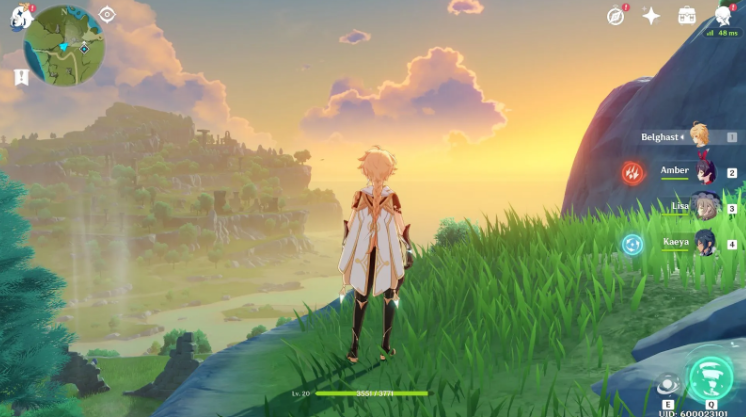
\includegraphics[scale=0.6]{UI1.png}
  \caption[UI example1]{ตัวอย่างที่ 1 UI ในเกมโดยอ้างอิงจากเกม genshin impact}
  \label{fig:UI1}
\end{figure}

\begin{figure}[htbp]
  \centering 
  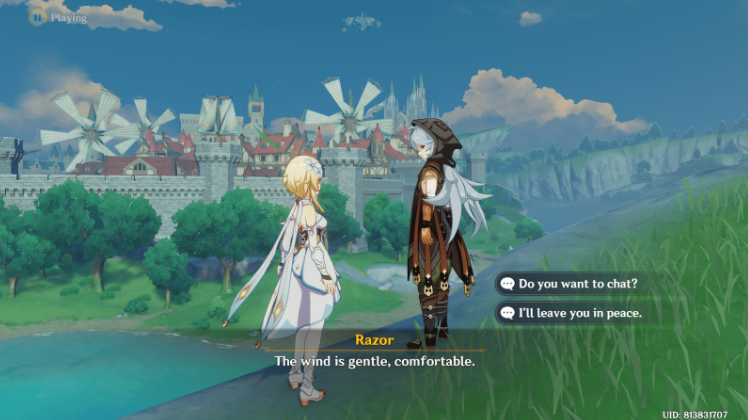
\includegraphics[scale=0.6]{UI2.png}
  \caption[UI example2]{ตัวอย่างที่ 2 UI ในเกมโดยอ้างอิงจากเกม genshin impact}
  \label{fig:UI2}
\end{figure}

%   `Oh, you wicked little thing!' cried Alice, catching up the
% kitten, and giving it a little kiss to make it understand that it
% was in disgrace.  `Really, Dinah ought to have taught you better
% manners!  You OUGHT, Dinah, you know you ought!' she added,
% looking reproachfully at the old cat, and speaking in as cross a
% voice as she could manage---and then she scrambled back into the
% arm-chair, taking the kitten and the worsted with her, and began
% winding up the ball again.  But she didn't get on very fast, as
% she was talking all the time, sometimes to the kitten, and
% sometimes to herself.  Kitty sat very demurely on her knee,
% pretending to watch the progress of the winding, and now and then
% putting out one paw and gently touching the ball, as if it would
% be glad to help, if it might.

%   `Do you know what to-morrow is, Kitty?' Alice began.  `You'd
% have guessed if you'd been up in the window with me---only Dinah
% was making you tidy, so you couldn't.  I was watching the boys
% getting in stick for the bonfire---and it wants plenty of
% sticks, Kitty!  Only it got so cold, and it snowed so, they had
% to leave off.  Never mind, Kitty, we'll go and see the bonfire
% to-morrow.'  Here Alice wound two or three turns of the worsted
% round the kitten's neck, just to see how it would look:  this led
% to a scramble, in which the ball rolled down upon the floor, and
% yards and yards of it got unwound again.

%   `Do you know, I was so angry, Kitty,' Alice went on as soon as
% they were comfortably settled again, `when I saw all the mischief
% you had been doing, I was very nearly opening the window, and
% putting you out into the snow!  And you'd have deserved it, you
% little mischievous darling!  What have you got to say for
% yourself?  Now don't interrupt me!' she went on, holding up one
% finger.  `I'm going to tell you all your faults.  Number one:
% you squeaked twice while Dinah was washing your face this
% morning.  Now you can't deny it, Kitty:  I heard you!  What that
% you say?' (pretending that the kitten was speaking.)  `Her paw
% went into your eye?  Well, that's YOUR fault, for keeping your
% eyes open---if you'd shut them tight up, it wouldn't have
% happened.  Now don't make any more excuses, but listen!  Number
% two:  you pulled Snowdrop away by the tail just as I had put down
% the saucer of milk before her!  What, you were thirsty, were you?

\subsection{หน้าหลัก(Main Menu) เป็นหน้าแรกที่เข้าเกมมาแล้วเจอหน้าเมนูนี้มีตัวเลือกดังนี้}
\begin{enumerate}
  \item New Game คือเริ่มเกมใหม่ตั้งแต่ต้น
  \item Continue เป็นการเล่นต่อจากที่เซฟไว้ล่าสุด
  \item Options คือการตั้งค่าตัวเกม เช่น ปรับระดับเสียง
  \item Exit คือการออกจากเกม
\end{enumerate}

\subsection{หน้าหยุดเกมชั่วคราว(Pause Menu) เมื่อเรากดปุ่มหยุดเกมชั่วคราวมีตัวเลือกดังนี้}
\begin{enumerate}
  \item Resume เล่นต่อ
  \item Options เหมือนกับในหน้าแรก จะมีการตั้งค่าภายในเกม
  \item Save and Exit เซฟเกมและกลับไปยังหน้าMain Menu
\end{enumerate}

\subsection{หน้าขณะเล่น(In Game UI) จะแสดงดังนี้}
\begin{enumerate}
  \item HP แสดงค่าพลังชีวิตของตัวละคร
  \item Rage แสดงจำนวนค่าความโกรธที่สะสมไว้แมื่อครบจะใช้ ultimate skill ได้
  \item Active Skills ที่ผู้เล่นจัดไว้ โดยจะแสดงว่าพร้อมใช้งานหรือว่าติดคูลดาวน์อยู่
  \item Ultimate Skill ที่ผู้เล่นจัดไว้ โดยจะแสดงว่าพร้อมใช้งานหรือว่าติดคูลดาวน์อยู่
  \item Character กดเพื่อเข้าไปยังหน้าต่างดู status ของผู้เล่น
  \item Inventory กดเพื่อเข้าไปหน้ากระเป๋าเพื่อจัดการไอเทมต่างๆ และจัดอาวุธที่นำมาใช้งาน
  \item Skills Menu กดเพื่อเข้าไปจัดสกิลเพื่อเอามาใช้งาน และปลดล็อคสกิลใหม่ๆ
  \item Quest กดเพื่อเข้าไปดูเควสต่างๆที่รับมาทั้งเควสหลัก หรือเควสเสริม
  \item Map แสดงจุดที่ผู้เล่นยืนอยู่ในแผนที่
  \item Pause Button กดหยุดเกมชั่วคราว
  \item Item shortcut ไอเทมที่เลือกไว้เพื่อกดใช้งานได้อย่างรวดเร็ว
\end{enumerate}

\subsection{หน้าพูดคุย(Talk UI) เมื่อมีการพูดคุยกับnpcหรือcut sceneที่มีการเล่าเนื้อเรื่อง}
\begin{enumerate}
\item Text แสดงข้อความคำพูดและผู้พูด
\item Answers ตัวเลือกคำพูดที่ผู้เล่นจะเลือกตอบตามสถานการณ์ 
\end{enumerate}

\section{Game System}
\subsection{ระบบค่าสถานะ(Character Status) }
ทั้งผู้เล่นและ monster จะมีค่าสถานะต่างๆที่ไม่เท่ากัน ขึ้นอยู่กับเลเวลและอุปกรณ์ที่สวมใส่อยู่
โดยค่าสถานะที่มีเฉพาะในผู้เล่นคือ Rage เป็นการสะสมความโกรธ มีค่าเพิ่มขึ้นเมื่อโจมตี monster สะสมค่าRageเพื่อใช้งานUltimate skill 
ส่วนค่าสถานะที่มีทั้งในผู้เล่นและ monster ได้แก่
\begin{enumerate}
\item Level เลเวลอัพแล้วจะมีค่าสถานะต่างๆสูงขึ้น และได้แต้มมาปลดล็อคสกิลของผู้เล่น
\item HP(พลังชีวิต)
\item Physical attack(พลังโจมตีกายภาพ)
\item Magic attack(พลังโจมตีเวท)
\item Physical Defence(พลังป้องกันกายภาพ)
\item Magic Defence(พลังป้องกันเวท)
\end{enumerate}

\subsection{ระบบสกิล(Skills System)}
ผู้เล่นสามารถปลดล็อคได้ผ่าน skill tree ได้แต้มมาปลดล็อคเมื่อเลเวลอัพ แต่ละสกิลมีเงื่อนไขการปลดล็อคที่ไม่เหมือนกัน สามารถเลือกสกิลที่ปลดล็อคแล้วมาจัดใส่ช่องใช้งานมีให้3ช่อง มีปุ่มกดแต่ละช่อง Q E และ R โดยใส่ Active Skills ได้2ช่อง Q E และ Ultimate Skill ได้ 1 ช่อง R

\subsection{ระบบไอเทม(Item System)}
ไอเทมแบ่งออกเป็น อุปกรณ์สวมใส่ ไอเทมที่ต้องกดใช้งาน และทอง

\begin{enumerate}
\item อุปกรณ์สวมใส่: อุปกรณ์แต่ละชิ้นจะบวกค่าสถานะให้ตัวละครไม่เท่ากัน และค่าสถานะดังกล่าวจะขึ้นอยู่กับเลเวลของอุปกรณ์ โดยไม่สามารถอัพเลเวลได้ และสามารถได้รับจากการดรอปของหลังจาก monster ตาย โดยแบ่งออกเป็น อาวุธ, ชุด, แหวน (ชุดและแหวนจะไม่แสดงให้เห็นที่ตัวละคร)
\item ไอเทมกดใช้งาน: เมื่อกดใช้งานจำนวนของไอเทมก็จะลดจำนวนลง ได้แก่ ยาฟื้นฟูเลือด, บัพชั่วคราว เช่นบัพ damage, defence  และมีช่อง item shortcut สามารถเลือกไอเทมกดใช้งานมาไว้ จะทำให้ใช้ไอเทมนั้นระหว่างต่อสู้ได้
\item ทอง: มีไว้สำหรับซื้อของที่ร้านค้า ซึ่งจะอยู่ในเมืองของมนุษย์ โดยร้านค้าจะขายอุปกรณ์สวมใส่ และไอเทมกดใช้งาน
\end{enumerate}

\subsection{ระบบอาวุธ(Weapon System)}
อาวุธที่ผู้เล่นใช้ได้มี 3 ประเภท คือ ดาบ ธนู หนังสือเวท ซึ่งอาวุธแต่ละประเภทจะมีเอกลักษณ์เฉพาะตัว เเละมี status ที่เพิ่มให้ผู้สวมใส่แตกต่างกันออกไป โดยผู้เล่นสามารถเปลี่ยนอาวุธระหว่างต่อสู้ได้ โดยอาวุธดังกล่าวจะต้องถูกสวมใส่อยู่เท่านั้น อาวุธอื่นๆที่ไม่ได้สวมใส่ไว้ จะไม่สามารถเปลี่ยนระหว่างการต่อสู้ไม่ได้ ซึ่งสวมใส่อาวุธได้ไม่เกิน 3 ชิ้น

\begin{enumerate}
\item ดาบ(Sword) คำนวณ damage จาก Physical attack ตีระยะใกล้ แรงสุด
\item ธนู(Bow) คำนวณ damage จาก Physical attack ตีระยะไกล
\item หนังสือเวท(Grimoire) คำนวณ damage  จาก Magic Attack ตีระยะไกลแบบ mini-aoe~\cite{aoe}
\end{enumerate}

\subsection{ระบบภารกิจ(Quest System)}
แบ่งออกเป็นสองประเภทได้แก่เควสหลักและเควสเสริม
\begin{enumerate}
\item เควสหลักหรือเควสเนื้อเรื่อง:  ผู้เล่นจะสามารถทำได้รอบเดียวต่อเควส เมื่อทำเควสแรกสำเร็จก็จะมีเควสต่อไปให้ทำเรื่อยๆ จนกว่าจะจบเนื้อเรื่องของเกม ในแต่ละเควสก็จะได้รับรางวัลต่างๆ ซึ่งแตกต่างกันในแต่ละเควส โดยจะมีการเล่าเนื้อเรื่องของเกมไปในตัว ในขณะทำเควสผู้เล่นจะไม่สามารถกดยกเลิกเควสได้
\item เควสรองหรือเควสเสริม: ผู้เล่นสามารถทำเควสได้หลายรอบ โดยจะเป็นการให้ผู้เล่นไปทำภารกิจต่างๆ เช่น ทำตามคำขอของเด็กน้อยให้ไปตามหาเพื่อนที่หลงในป่า เป็นต้น ในการทำเควสรอง เมื่อทำเควสสำเร็จ ผู้เล่นจะได้ค่าประสบการณ์ เงินหรือไอเทมเป็นรางวัล และผู้เล่นสามารถกดยกเลิกเควสได้
\end{enumerate}

\subsection{ระบบมอนสเตอร์(Monster System)}
แบ่งออกเป็นสามประเภทได้แก่
\begin{enumerate}
\item Normal monsters : พบเจอได้ทั่วไปในแมพบริเวณนอกเมือง monster แต่ละพื้นที่จะมีเลเวล และค่าสถานะไม่เหมือนกันขึ้นกับสถานที่และอื่นๆ monster มีขอบเขต และเส้นทางการเดินของตัวเอง เมื่อ monster พบผู้เล่น monster จะทำการโจมตีใส่ผู้เล่น ถ้าผู้เล่นเดินหนีออกนอกเขตได้ก็จะเลิกไล่ตามแล้วกลับไปจุดของตัวเอง พร้อมกับรีเซ็ตเลือดตัวเองด้วย ซึ่งหาก monster ตายมันจะเกิดใหม่เมื่อผ่านไประยะเวลาหนึ่ง นานมากน้อยแค่ไหนขึ้นอยู่กับชนิด เเละเลเวลของ monster นั้นๆ
\item Zone’s Boss : พบในแต่ละพื้นที่ของเกม โดยพบได้เพียงตัวเดียวต่อพื้นที่เท่านั้น ซึ่งทั้งเกมจะมีทั้งหมดสามตัว แต่ละตัวจะประจำตำแหน่งในพื้นที่ต่างๆของใครของมัน ได้เเก่ พื้นที่ป่าไม้, ทะเลทราย และ ป่าหิมะ สามารถฆ่าได้ครั้งเดียว เมื่อฆ่าได้จะดรอปแหวนแห่งพลังที่เมื่อรวบรวมครบสามวง แหวนทั้งสามจะรวมกันกลายเป็นสุดยอดแหวน ซึ่งใช้ในการทำลายบาเรียของทวีปของจอมมาร ทำให้ผู้เล่นสามารถบุกเข้าไปต่อสู้ในทวีปของจอมมารได้
\item Demon King : มีเพียงตัวเดียวในเกม เป็นบอสสุดท้ายของเกม ถ้าผู้เล่นสามารถเอาชนะจอมมารได้ เกมก็จะจบ Demon King มีจะความสามารถที่หลากหลาย พลังป้องกันสถานะต่างๆสูง ต้องใช้ทักษะการเล่น และตัวละครที่เลเวลค่อนข้างสูง
\\
\\
\\
\\
\end{enumerate}


\section{ตัวละคร}
\subsection{ผู้เล่น}
ตัวละครหลักของเกมจะเป็นเด็กผู้หญิง ดังรูป
\begin{figure}[htbp]
  \centering 
  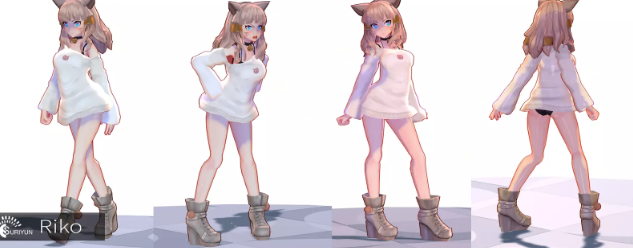
\includegraphics[scale=0.8]{player.png}
  \caption[player]{ตัวอย่างตัวละครของผู้เล่น}
  \label{fig:player}
\end{figure}

% \begin{center}
% \includegraphics{800px-Briny_Beach.jpg}
% \end{center}

\subsection{Normal Monster}
Monster ในเกมจะมีหลากหลายประเภท โดยแบ่งหลักเป็น สามารถบินได้กับไม่สามารถบิน ดังรูป
\begin{figure}[htbp]
  \centering 
  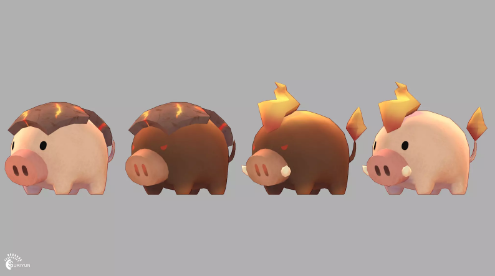
\includegraphics[scale=0.8]{mon1.png}
  \caption[Normal Monster1]{ตัวอย่างที่ 1 Normal Monster}
  \label{fig:NormalMon1}
\end{figure}

\begin{figure}[htbp]
  \centering 
  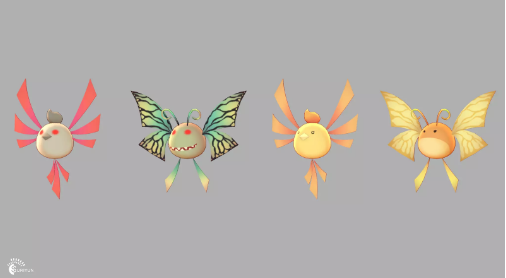
\includegraphics[scale=0.8]{mon2.png}
  \caption[Normal Monster2]{ตัวอย่างที่ 2 Normal Monster}
  \label{fig:NormalMon2}
\end{figure}


\subsection{Zone’s Boss}
Zone’s Boss ในเกมจะมีเพียง 3 ตัว ซึ่งมีรูปร่างแตกต่างกันไป
\begin{figure}[htbp]
  \centering 
  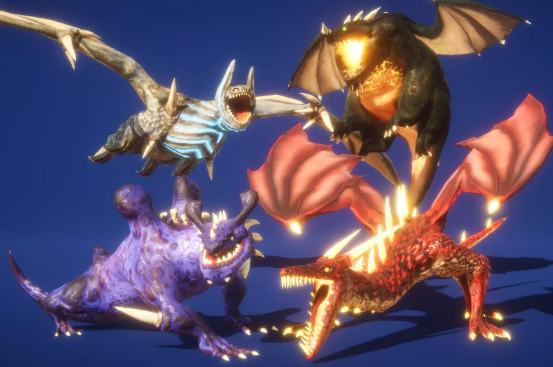
\includegraphics[scale=0.6]{boss.png}
  \caption[Zone’s Boss]{ตัวอย่างที่ Zone’s Boss}
  \label{fig:ZoneBoss }
\end{figure}
  

\subsection{Demon King}
Demon King ในเกมจะมีเพียง 1 ตัว เมื่อชนะได้ก็จะจบเกม
\begin{figure}[htbp]
  \centering 
  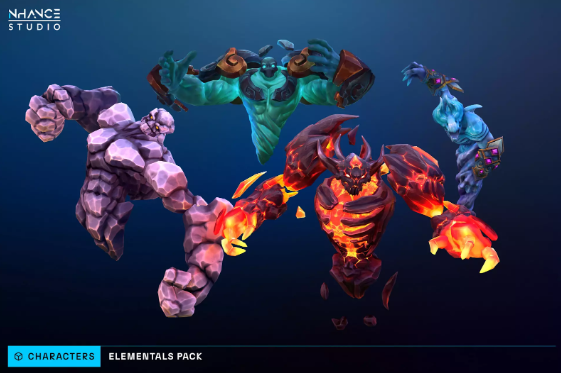
\includegraphics[scale=0.6]{demon.png}
  \caption[Demon King]{ตัวอย่างที่ Demon King}
  \label{fig:DemonKing }
\end{figure}

\section{Game play}
\subsection{การควบคุมตัวละคร}
การควบคุมตัวละครในโครงงานนี้มีความสำคัญต่อความน่าสนใจ ความสนุก และการพลิกแพลง
ภายในเกม เนื่องจากต้องใช้ความชำนาญ และไหวพริบในการควบคุม โดยสามารถอธิบายรายละเอียดการ
ควบคุมตัวละครด้วยคีย์บอร์ดดังนี้
\begin{enumerate}
\item W A S D ใช้สำหรับการเดินหน้า ซ้าย ถอยหลัง และขวาตามลำดับ
\item Space bar ใช้ในการกระโดด
\item Mouse Left Click ใช้สำหรับโจมตีปกติ
\item Mouse Right Click ใช้สำหรับการโจมตีหนัก
\item Q, E ใช้งานActive Skills ที่เลือกไว้ 2 สกิล ตามลำดับ
\item R ใช้งานUltimate Skill
\item Left Alt ใช้เพื่อนำcursorออกมาจากการควบคุมมุมมองตัวละคร เพื่อนำมากดเมนูต่างๆ
\item Scroll Wheel ใช้เพื่อเปลี่ยนอาวุธในการต่อสู้
\item Left Shift ใช้เพื่อทำการพุ่งไปในทิศทางที่ควบคุมอยู่
\end{enumerate}

\subsection{ระบบการต่อสู้}
มีการต่อสู้กับ monster ภายในเกม โดยเมื่อทำความเสียหายใส่ monster จนพลังชีวิตของมันหมด ผู้เล่นก็จะได้รับค่าประสบการณ์(Exp)และมีโอกาสสุ่มได้รับไอเทมที่มีเลเวลใกล้เคียงกับ monster นั้นและเงิน โดยถ้าเป็น zone’s boss ก็จะดรอปไอเทมพิเศษที่จำเป็นสำหรับการทำเควสเนื้อเรื่องด้วย
\subsection{เป้าหมายการเล่นเกม}
ทำเควสเนื้อเรื่องไปเรื่อยๆระหว่างนั้นจะทำเควสรองหรือว่าสำรวจโลกเองก็ได้
โดยเควสเนื้อเรื่องจะให้ตัวหลักเดินทางไปยังพื้นที่ต่างๆ 3โซนคือป่า น้ำแข็ง ทะเลทราย เพื่อปราบมินิบอสของโซนนั้นและได้รับแหวนที่เพิ่มพลังผู้สวมใส่ เมื่อรวบรวมแหวนครบ3วง แหวนก็จะรวมกันเป็นสุดยอดแหวนที่สามารถทำลายบาเรียที่ปกป้องจอมมารอยู่ ทำให้ผู้เล่นสามารถโจมตีจอมมารได้ เมื่อชนะจอมมารได้ก็จะจบเกม

\subsection{แผนที่}
จะแบ่งออกเป็นสองทวีปโดย ฝั่งซ้ายเป็นที่อยู่ของมนุษย์ แบ่งเป็น 3 ภูมิภาคใหญ่ๆ คือ ป่า ทะเลทราย และป่าหิมะ มีเมืองหลวงอยู่ตรงกลาง ฝั่งขวาเป็นที่อยู่ของจอมมารและลูกน้องพื้นที่ส่วนใหญ่เป็นลาวาและฝุ่นควัน



  
  

